\documentclass[a4paper,10pt]{article}
\usepackage[utf8]{inputenc}
\usepackage{graphicx}

%opening
\title{Antenna Array Position Calibration for the Transient Array Radio Telescope}
\author{Timothy C.A. Molteno}

\begin{document}

\maketitle

\begin{abstract}
The Transient Array Radio Telescope is an all-sky radio telescope designed to detect transient events. The antenna array contains 24 elements. For interferometric imaging, the positions of these antennas must be accurately known. This paper presents the technique used to calibrate the antenna positions. The technique is iterative, based on a least-squares minimization that reports outliers that are then re-measured. This technique is robust, can be performed with simple equipment and provides accuracy to within 0.01 wavelengths -- sufficent for interferometic imaging.
\end{abstract}

\section{Background and Introduction}

The Transient Array Radio Telescope (TART) is an all-sky imaging interferometer that operates in the L1 band. The project is open-source and has been deployed widely as a tool for detect radio transients, and also as a platform for the development of new radio imaging algorithms. TART telescopes are often installed as part of a week-long workshop that introduces the attendees to radio astronomy, radio imaging and interferometry, and at the same time, assembles and installs a TART radio telescope. The position calibration process for the antenna array must determine the relative locations of the antennas to within $\approx 5$mm in the coordinate system of the phase center of the antenna array.

\begin{figure}
 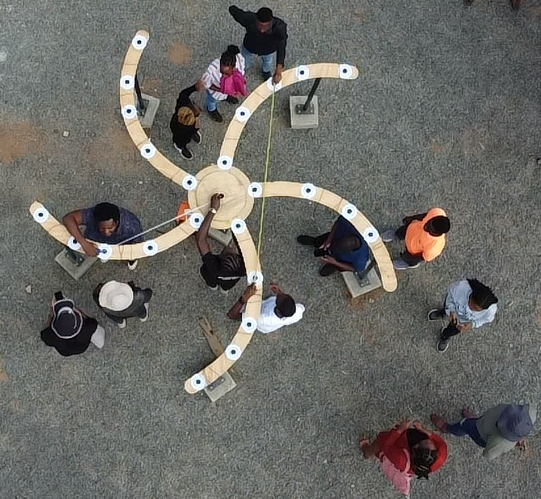
\includegraphics[width=\linewidth]{fig/botswana_calibration.png}
 \caption{Aerial view of a TART being calibrated by attendees at a TART workshop hosted at the Botswana International University of Science and Technology, in March 2025.}
\end{figure}

The calibration process must involve easy-to-make measurements, and be robust to accidental errors in measurement. This paper outlines an iterative calibration process that meets these requirements.

\section{Method}

The process involves measuring two distances. The first are the {\em radial distances} between the phase-centre and the centre of each antenna. There are 24 radial distance measurements $r_i$. The second measurements are the pairwise distances between each pair of antennas. There are $\frac{1}{2} N (N-1)$ unique pairs of antennas for an array with $N$ antennas. For the TART there are 276 pairwise distances $\delta_{ij}$ between antennas $i$ and $j$. As the measurements do not constrain the global rotation of the array, it is assumed that the direction between the phase centre and one of the antennas is known. This direction is the measured angle between one antenna and geographic North.

The purpose of the algorithm is to estimate the 24 antenna positions in the $x-y$ plane that are most consistent with the measurements.

\subsection{Least Squares Estimator}

Given a set, $x,y$ of 24 antenna positions, and the $r_i, \delta_{ij}$, we form a least-squares estimator

\begin{eqnarray}
 L_{}(x, y, r, \delta) & = & \sum_{i=1}^{N} \left( r_i - \sqrt{x_{i,0}^2 + y_i^2}  \right)^2 \nonumber \\
 & + & \sum_{i,j=1}^{N} \left( \delta_{ij} - \sqrt{(x_i - x_j)^2 + (y_i - y_j^2}  \right)^2
\end{eqnarray}


\end{document}
